\subsection*{\textbf{Erläuterung des Punktesystems}}\label{Erläuterung des Punktesystems} 
Um die verschiedenen Optionen möglichst gut vergleichbar zu machen, hatten wir uns ein Punktesystem mit einer maximalen Punktzahl von 5 pro Evaluierungskriterium definiert. Dabei hatten die einzelnen Punkte keine feste Bedeutung, sondern sollten lediglich die einzelnen Optionen untereinander bezüglich Eignung vergleichbar machen. Je höher das erreichte Endergebnis der einzelnen Optionen, umso mehr hatten wir die Option für die Umsetzung in Erwägung gezogen. Wichtig hierbei war, dass bei dem Evaluierungskriterium „Komplexität“ eine hohe Komplexität als negativ gewertet wurde und demzufolge eine geringere Punktzahl vergeben wurde. Bei den restlichen Evaluierungskriterien war das Gegenteil der Fall. So führten beispielsweise eine hohe Skalierbarkeit/Erweiterbarkeit, ein hoher Erfüllungsgrad der Anforderungen, ein gutes Preis-/Nutzen-Verhältnis der Option zu einem besseren Endergebnis. Das Endergebnis pro Option wurde schlussendlich aus dem arithmetischen Mittel der vier Teilergebnisse aus den Evaluierungskriterien berechnet.

\subsection*{\textbf{Ergebnis \& Diskussion}}\label{Ergebnis & Diskussion} 
Die Tabelle \ref{fig:Auswertung der einzelnen Optionen} zeigt das Ergebnis unserer Auswertung für die einzelnen Optionen. Die Auswertung zeigt, dass Option 1 am wenigsten komplex war und demzufolge am einfachsten und schnellsten bei einer Eigenentwicklung umzusetzen war, da hierbei lediglich eine API entwickelt werden würde, welches auf die Drittsysteme zugreift. Dies mag zwar eine preisgünstige Option sein, jedoch war die Lösung auf Grund der engen Kopplung zwischen den Systemen nicht einfach skalierbar/erweiterbar. Folglich war der Erfüllungsgrad der Anforderungen von Statistance sehr gering, da ein hoher Wert auf Skalierbarkeit/Erweiterbarkeit und Flexibilität bei der Lösung gelegt wurde. Bei Option 2 wurde eine höhere Skalierbarkeit und Performance als Option 1 durch die Einführung einer separaten Datenbank erreicht, welches dadurch ein besseres Preis-/Nutzen-Verhältnis hatte.  Allerdings bestand weiterhin eine enge Kopplung zwischen den Systemen und die Anforderungen konnten nur mittelmäßig abgedeckt werden. Die enge Kopplung zwischen den Systemen wurde schlussendlich mit Option 3 beseitigt und bot durch das Konzept mit Integration Flows und Integration Components eine sehr gute Skalierbarkeit/Erweiterbarkeit an und war aus funktionaler Sicht dabei auch am fortgeschrittensten unter allen Optionen. Folglich wäre der Entwicklungs-/Wartungsaufwand dort am geringsten gewesen und hätte auch die Gesamtanforderungen von Statistance abgedeckt. Auf der anderen Seite war das OIH in Bezug auf Infrastruktur sowie Setup unter allen Lösungen am komplexesten und Statistance hatte derzeit nur einen Teil der Services benötigt. Hinzu kam, dass der Kunde von Statistance noch nicht bereit für die Cloud war und wenig Erfahrung beim Betrieb mit Cloud-Technologien hatte. Dementsprechend war das Preis-/Nutzen-Verhältnis für Option 3 eher mittelmäßig, da nicht alle Services derzeit benötigt waren, aber trotzdem die Kosten für den Betrieb der essentiellen Services getragen hätte werden müssen. Schlussendlich hatten wir mit Option 4 eine Lösung geschaffen, die eine ähnliche Skalierbarkeit/Erweiterbarkeit wie das OIH erreicht hatte, jedoch im Vergleich weniger standardisiert war. Die Komplexität des Systems war zwar höher als Option 1 und Option 2, jedoch war diese geringer als bei Option 3 in Bezug auf Betrieb und Setup. Auf Grund der Tatsache, dass bei Option 4 jedoch nur relevante Services für Statistance vorgesehen waren, hatte diese Lösung ein ideales Preis-/Nutzen-Verhältnis und konnte somit auch alle Anforderungen von Statistance abdecken. Schließlich hatte Option 4 bei der Auswertung am besten abgeschnitten, weshalb wir uns für diese Lösung entschieden haben. 

\begin{table}[!h]
    \centering
    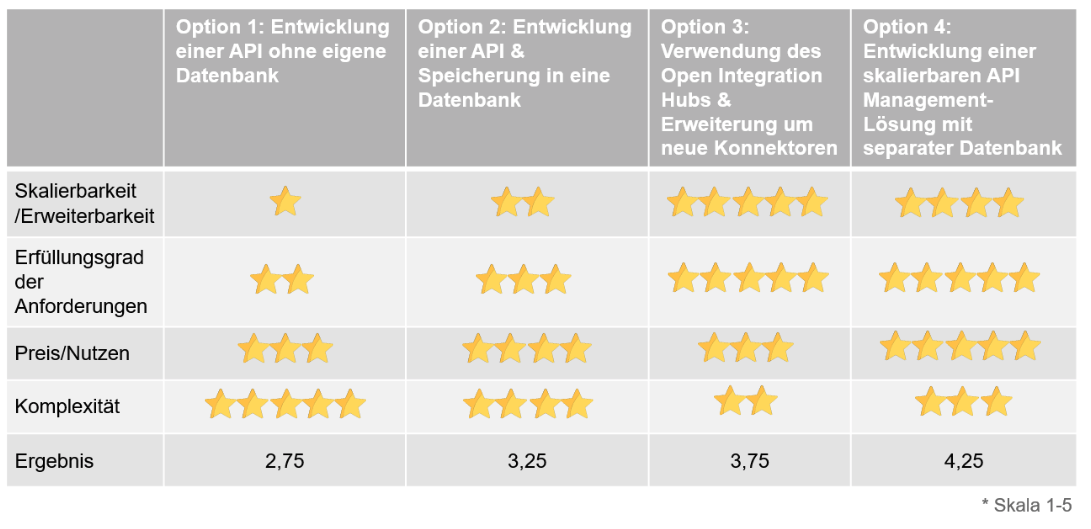
\includegraphics[width=15cm]{images/0x_implementation_possibilities/results.png}
    \caption{Auswertung der einzelnen Optionen}
    \label{fig:Auswertung der einzelnen Optionen}
\end{table}